\chapter{Visión General del proyecto}

El propósito de este proyecto es desplegar toda la infraestructura de la empresa AlterAid en un dispositivo móvil, en nuestro caso una Raspberry Pi, con la finalidad de poder conseguir desplegar las aplicaciones en lugares remotos, sin conexión a internet y/o que han sufrido un desastre natural.

Como segundo objetivo del proyecto queremos implementar un pequeño despliegue de sensores haciendo que nuestra Raspberry Pi sea el nodo central o sumidero de datos. Para poder llevar a cabo todo esto es necesario contar con la utilización de los contenedores usando la tecnología Docker. Puesto que éstos nos facilitarán el trabajo, su utilización fuera del mundo de servidores es motivo de investigación.

\section{Docker}

La idea detrás de Docker es crear contenedores ligeros y portables para las aplicaciones software que puedan ejecutarse en cualquier máquina con Docker instalado, independientemente del sistema operativo que la máquina tenga por debajo, facilitando así también los despliegues.

\begin{figure}[htb]
\begin{center}
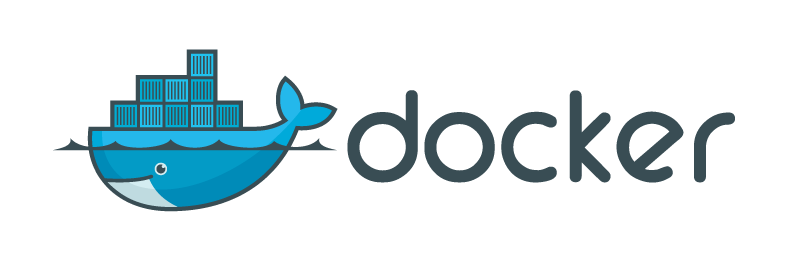
\includegraphics[width=0.5\textwidth]{./setup/dockerLogo}
\caption{Logotipo de Docker}
\label{F:prova}
\end{center}
\end{figure}


\section{Aaaida}
Es una plataforma desarrollada por la empresa AlterAid que nos permite crear un usuario y con este usuario poder tener varios vínculos. Un Vínculo es un ente que representa aquello por el que el Usuario se ocupa y preocupa. Ejemplos de Vínculos de Usuario pueden ser familiares, pacientes, amigos, etc. 
Esta es una plataforma web la cual recoge todos los datos de las aplicaciones de la empresa y los almacena. Por eso la importancia de poder desplegar toda la infraestructura en un dispositivo que sea fácil de transportar y poder llegar a cualquier lugar.
\newpage
\begin{figure}[htb]
\begin{center}

\includegraphics[width=0.5\textwidth]{./setup/aaaidaLogo}
\caption{Logotipo de Aaaida}
\label{F:prova}
\end{center}
\end{figure}





\section{Motivación}

Conseguir el despliegue de toda la infraestructura de una empresa en un dispositivo de reducidas prestaciones y tamaño como seria una Raspberry Pi permitiría la apertura de nuevos campos de investigación y de mercado puesto que se podrían desarrollar otro tipo de aplicaciones para casos de emergencia o lugares con pocos medios. 
Utilizar una tecnología de servidores como es Docker conlleva un gran avance en el mundo de Internet of Things (de ahora en adelante IoT).
El presente proyecto representa una prueba de concepto para versiones futuras en las cuales se podrían utilizar estas tecnologías para facilitar el despliegue tanto de las aplicaciones como de sus actualizaciones ya que al utilizar Docker solo se debería actualizar el contenedor independiente y no todo el sistema.
\section{Objetivos}

Los objetivos fijados para el desarrollo de este proyecto son los siguientes:

\begin{itemize}
\item Analizar y escoger las tecnologías a utilizar para el desarrollo del proyecto
\item La instalación de Docker en una Raspberry Pi
\item El despliegue de la infraestructura de la empresa AlterAid
\item La creación de pequeños nodos
\item El despliegue de la red
\item Contemplar la viabilidad de creación de redes smart con estas tecnologías. 
\end{itemize}
\pagebreak

\section{Organización del proyecto}

En primer lugar, para poder cumplir todos los puntos de los objetivos necesitaremos estudiar un poco más a fondo todas las tecnologías que se utilizarán a lo largo de todo el proyecto. Serán explicadas en sus respectivos capítulos.

Como se ha explicado previamente se utilizará una Raspberry Pi, donde se desplegará la aplicación mediante Docker. Para poder llevarlo a cabo se tendrán que estudiar las diferentes posibilidades como, por ejemplo, si es posible ejecutar Docker en un sistema ARM o si se podrá virtualizar la Raspberry para poder hacer las pruebas de una manera más cómoda. Todo esto se podrá ver en el capítulo 2 y capítulo 3.

Una vez desplegada y ejecutada la aplicación es necesario arrancar Aaaida. En el capítulo 4 se podrá ver una pequeña explicación del funcionamiento de la plataforma y sus funcionalidades. 

Para terminar la parte técnica, vendría el paso de crear la red de sensores y
comunicarnos con la Raspberry. Una vez se haya llevado a cabo esta conexión, se realizará el envío de los datos y su correcto almacenamiento. En el capítulo 5 se comentará como hacerlo para poder ser visualizados en la plataforma Aaaida. 

Por último, con la plataforma en la Raspberry y la red de sensores funcionando obtendremos el último capítulo donde se podrán ver las conclusiones y resultados sobre la viabilidad de este proyecto.
